\documentclass[10pt,a4paper]{book}
\usepackage{lmodern}
\usepackage{amssymb,amsmath}
\usepackage{ifxetex,ifluatex}
\usepackage{fixltx2e} % provides \textsubscript
\ifnum 0\ifxetex 1\fi\ifluatex 1\fi=0 % if pdftex
  \usepackage[T1]{fontenc}
  \usepackage[utf8]{inputenc}
\else % if luatex or xelatex
  \ifxetex
    \usepackage{mathspec}
  \else
    \usepackage{fontspec}
  \fi
  \defaultfontfeatures{Ligatures=TeX,Scale=MatchLowercase}
\fi
% use upquote if available, for straight quotes in verbatim environments
\IfFileExists{upquote.sty}{\usepackage{upquote}}{}
% use microtype if available
\IfFileExists{microtype.sty}{%
\usepackage[]{microtype}
\UseMicrotypeSet[protrusion]{basicmath} % disable protrusion for tt fonts
}{}
\PassOptionsToPackage{hyphens}{url} % url is loaded by hyperref
\usepackage[unicode=true]{hyperref}
\PassOptionsToPackage{usenames,dvipsnames}{color} % color is loaded by hyperref
\hypersetup{
            pdftitle={Estatística Computacional com R},
            pdfauthor={Fernando P. Mayer; Wagner H. Bonat},
            colorlinks=true,
            linkcolor=Maroon,
            citecolor=Blue,
            urlcolor=Blue,
            breaklinks=true}
\urlstyle{same}  % don't use monospace font for urls
\usepackage[margin=3cm]{geometry}
\usepackage{color}
\usepackage{fancyvrb}
\newcommand{\VerbBar}{|}
\newcommand{\VERB}{\Verb[commandchars=\\\{\}]}
\DefineVerbatimEnvironment{Highlighting}{Verbatim}{commandchars=\\\{\}}
% Add ',fontsize=\small' for more characters per line
\usepackage{framed}
\definecolor{shadecolor}{RGB}{248,248,248}
\newenvironment{Shaded}{\begin{snugshade}}{\end{snugshade}}
\newcommand{\KeywordTok}[1]{\textcolor[rgb]{0.13,0.29,0.53}{\textbf{#1}}}
\newcommand{\DataTypeTok}[1]{\textcolor[rgb]{0.13,0.29,0.53}{#1}}
\newcommand{\DecValTok}[1]{\textcolor[rgb]{0.00,0.00,0.81}{#1}}
\newcommand{\BaseNTok}[1]{\textcolor[rgb]{0.00,0.00,0.81}{#1}}
\newcommand{\FloatTok}[1]{\textcolor[rgb]{0.00,0.00,0.81}{#1}}
\newcommand{\ConstantTok}[1]{\textcolor[rgb]{0.00,0.00,0.00}{#1}}
\newcommand{\CharTok}[1]{\textcolor[rgb]{0.31,0.60,0.02}{#1}}
\newcommand{\SpecialCharTok}[1]{\textcolor[rgb]{0.00,0.00,0.00}{#1}}
\newcommand{\StringTok}[1]{\textcolor[rgb]{0.31,0.60,0.02}{#1}}
\newcommand{\VerbatimStringTok}[1]{\textcolor[rgb]{0.31,0.60,0.02}{#1}}
\newcommand{\SpecialStringTok}[1]{\textcolor[rgb]{0.31,0.60,0.02}{#1}}
\newcommand{\ImportTok}[1]{#1}
\newcommand{\CommentTok}[1]{\textcolor[rgb]{0.56,0.35,0.01}{\textit{#1}}}
\newcommand{\DocumentationTok}[1]{\textcolor[rgb]{0.56,0.35,0.01}{\textbf{\textit{#1}}}}
\newcommand{\AnnotationTok}[1]{\textcolor[rgb]{0.56,0.35,0.01}{\textbf{\textit{#1}}}}
\newcommand{\CommentVarTok}[1]{\textcolor[rgb]{0.56,0.35,0.01}{\textbf{\textit{#1}}}}
\newcommand{\OtherTok}[1]{\textcolor[rgb]{0.56,0.35,0.01}{#1}}
\newcommand{\FunctionTok}[1]{\textcolor[rgb]{0.00,0.00,0.00}{#1}}
\newcommand{\VariableTok}[1]{\textcolor[rgb]{0.00,0.00,0.00}{#1}}
\newcommand{\ControlFlowTok}[1]{\textcolor[rgb]{0.13,0.29,0.53}{\textbf{#1}}}
\newcommand{\OperatorTok}[1]{\textcolor[rgb]{0.81,0.36,0.00}{\textbf{#1}}}
\newcommand{\BuiltInTok}[1]{#1}
\newcommand{\ExtensionTok}[1]{#1}
\newcommand{\PreprocessorTok}[1]{\textcolor[rgb]{0.56,0.35,0.01}{\textit{#1}}}
\newcommand{\AttributeTok}[1]{\textcolor[rgb]{0.77,0.63,0.00}{#1}}
\newcommand{\RegionMarkerTok}[1]{#1}
\newcommand{\InformationTok}[1]{\textcolor[rgb]{0.56,0.35,0.01}{\textbf{\textit{#1}}}}
\newcommand{\WarningTok}[1]{\textcolor[rgb]{0.56,0.35,0.01}{\textbf{\textit{#1}}}}
\newcommand{\AlertTok}[1]{\textcolor[rgb]{0.94,0.16,0.16}{#1}}
\newcommand{\ErrorTok}[1]{\textcolor[rgb]{0.64,0.00,0.00}{\textbf{#1}}}
\newcommand{\NormalTok}[1]{#1}
\usepackage{longtable,booktabs}
% Fix footnotes in tables (requires footnote package)
\IfFileExists{footnote.sty}{\usepackage{footnote}\makesavenoteenv{long table}}{}
\IfFileExists{parskip.sty}{%
\usepackage{parskip}
}{% else
\setlength{\parindent}{0pt}
\setlength{\parskip}{6pt plus 2pt minus 1pt}
}
\setlength{\emergencystretch}{3em}  % prevent overfull lines
\providecommand{\tightlist}{%
  \setlength{\itemsep}{0pt}\setlength{\parskip}{0pt}}
\setcounter{secnumdepth}{5}
% Redefines (sub)paragraphs to behave more like sections
\ifx\paragraph\undefined\else
\let\oldparagraph\paragraph
\renewcommand{\paragraph}[1]{\oldparagraph{#1}\mbox{}}
\fi
\ifx\subparagraph\undefined\else
\let\oldsubparagraph\subparagraph
\renewcommand{\subparagraph}[1]{\oldsubparagraph{#1}\mbox{}}
\fi

% set default figure placement to htbp
\makeatletter
\def\fps@figure{htbp}
\makeatother

%%----------------------------------------------------------------------
%% Opções comuns
\usepackage[brazil]{babel}
\usepackage[T1]{fontenc}
\usepackage{amsmath,amsfonts,amssymb,amsthm}
%%----------------------------------------------------------------------

%%----------------------------------------------------------------------
%% FLOATS: graficos e tabelas
\usepackage{graphicx}
%%----------------------------------------------------------------------

%%----------------------------------------------------------------------
%% hyperref e xcolor
\usepackage{hyperref} % hidelinks
\usepackage{xcolor}
\hypersetup{
    colorlinks,
    linkcolor={red!50!black},
    citecolor={blue!50!black},
    urlcolor={blue!80!black}
}
%%----------------------------------------------------------------------

%%----------------------------------------------------------------------
%% FONTES
%% micro-tipografia
% \usepackage[protrusion=true,expansion=true]{microtype}
%% Bitstream Charter with mathdesign
%\usepackage{lmodern} % sans-serif: Latin Modern
% \usepackage[charter]{mathdesign} % serif: Bitstream Charter
%\usepackage[scaled]{beramono} % truetype: Bistream Vera Sans Mono
% \usepackage[scaled]{helvet}
\usepackage{mathpazo}
\usepackage{inconsolata}
%%----------------------------------------------------------------------

\title{Estatística Computacional com R}
\author{Fernando P. Mayer \and Wagner H. Bonat}
\date{Laboratório de Estatística e Geoinformação (LEG)\\
Departamento de Estatística (DEST)\\
Universidade Federal do Paraná (UFPR)\\[2\baselineskip]2018-07-24\\
Última atualização: 2018-07-24}

\begin{document}
\maketitle

{
\hypersetup{linkcolor=black}
\setcounter{tocdepth}{2}
\tableofcontents
}
\chapter*{Prefácio}\label{prefacio}


Alguma coisa aqui.

\chapter{Computação científica e interação com o
R}\label{computacao-cientifica-e-interacao-com-o-r}

\section{Interagindo com o
computador}\label{interagindo-com-o-computador}

O que significa este ícone?

\begin{center}
\includegraphics[width=0.5\linewidth]{img/excelcsvgrey} \end{center}

\begin{itemize}
\tightlist
\item
  É um documento do Microsoft Excel?
\item
  É um arquivo de \textbf{texto pleno}, separado por vírgulas (CSV
  \emph{comma separated values})
\item
  De fato, o nome do arquivo é \texttt{final.csv} e não \texttt{final}
\item
  O Excel pode sim abrir este arquivo\ldots{} assim como milhares de
  outros programas!
\end{itemize}

O que está acontecendo?

\begin{itemize}
\tightlist
\item
  O computador (leia-se, nesse caso, o sistema operacional Windows)
  ``proteje'' o usuário dos detalhes sujos
\item
  Isso é ruim? \textbf{Sim!}
\item
  O usuário se acostuma com o computador ditando as regras
\item
  É importante lembrar que é você quem deve dizer o que o computador
  deve fazer (nesse caso, com qual programa abrir certo arquivo)
\end{itemize}

O que deve acontecer?

\begin{itemize}
\tightlist
\item
  Para a maioria dos usuários, a interação com o computador se limita a
  clicar em links, selecionar menus e caixas de diálogo
\item
  O problema com essa abordagem é que parece que o usuário é controlado
  pelo computador
\item
  A verdade deve ser o oposto!
\item
  É o usuário que possui o controle e deve dizer para o computador
  exatamente o que fazer
\item
  Escrever código ainda tem a vantagem de deixar registrado tudo o que
  foi feito
\end{itemize}

\section{Editores de texto}\label{editores-de-texto}

Uma característica importante de códigos de programação é que eles são
em \textbf{texto puro}, por isso precisamos de um bom \textbf{editor de
textos}

Características de um bom editor:

\begin{itemize}
\tightlist
\item
  \textbf{Identação automática}
\item
  \textbf{Complementação de parênteses}
\item
  \textbf{Destaque de sintaxe} (\emph{syntax highlighting})
\item
  \textbf{Numeração de linhas}
\item
  \textbf{Auto completar comandos}
\end{itemize}

\subsection{Editores para R}\label{editores-para-r}

Windows:

\begin{itemize}
\tightlist
\item
  Interface padrão: pouco recomendado
\item
  Tinn-R
\end{itemize}

Linux:

\begin{itemize}
\tightlist
\item
  Vim-R-plugin
\item
  Gedit-R-plugin
\end{itemize}

Todas as plataformas:

\begin{itemize}
\tightlist
\item
  Rstudio: recomendado para iniciantes
\item
  Emacs + ESS: altamente recomendado
\end{itemize}

\section{R}\label{r}

\begin{quote}
\emph{``The statistical software should help, by supporting each step
from user to programmer, with as few intrusive barriers as possible.''}
\end{quote}

\begin{quote}
\emph{``\ldots{} to turn ideas into software, quickly and faithfully.''}
\end{quote}

--- John M. Chambers

O R é um dialeto do S e:

\begin{itemize}
\item
  \emph{Ambiente} estatístico para análise de dados e produção de
  gráficos
\item
  Uma completa linguagem de programação:

  \begin{itemize}
  \tightlist
  \item
    Interpretada (contrário de compilada)
  \item
    Orientada a objetos:
  \end{itemize}

  \emph{Tudo no R é um objeto\ldots{}}
\item
  Livre distribuição (código-aberto)
\item
  Mais de 10000 pacotes adicionais
\end{itemize}

Pequeno histórico:

\begin{itemize}
\tightlist
\item
  1980: Linguagem S: desenvolvida por R. Becker, J. Chambers e A. Wilks
  (AT\&T Bell Laboratories)
\item
  1980: Versão comercial: S-Plus (Insightful Corporation)
\item
  1996: Versão livre: R desenvolvido por R. Ihaka e R. Gentleman
  (Universidade de Auckland)
\item
  1997: R Development Core Team
\item
  Hoje: 20 desenvolvedores principais e muitos outros colaboradores em
  todo o mundo
\item
  Estatísticos, matemáticos e programadores
\end{itemize}

\subsection{Configuração inicial}\label{configuracao-inicial}

\begin{itemize}
\item
  O \textbf{diretório de trabalho} é uma pasta onde o R será
  direcionado. Todos os arquivos que serão importados (base de dados,
  \ldots{}) ou exportados (base de dados, gráficos, \ldots{}) por ele
  ficarão nesta pasta.
\item
  Existem duas maneiras de configurar o diretório de trabalho (suponha
  que vamos usar a pasta \texttt{\textasciitilde{}/estatcomp1}):
\item
  \texttt{1)} Utilizando a função \texttt{setwd()} dentro do R:
\end{itemize}

\begin{Shaded}
\begin{Highlighting}[]
\KeywordTok{setwd}\NormalTok{(}\StringTok{"~/estatcomp1"}\NormalTok{)}
\end{Highlighting}
\end{Shaded}

\begin{itemize}
\tightlist
\item
  \texttt{2)} Pelo menu do RStudio em
  \texttt{Session\ \textgreater{}\ Set\ Working\ Directory\ \textgreater{}\ Choose\ Directory...}
  Confira o diretório que está trabalhando com a função
\end{itemize}

\begin{Shaded}
\begin{Highlighting}[]
\KeywordTok{getwd}\NormalTok{()}
\end{Highlighting}
\end{Shaded}

\subsection{O R como uma calculadora}\label{o-r-como-uma-calculadora}

O símbolo \texttt{\textgreater{}} indica que o R está pronto para
receber um comando:

\begin{Shaded}
\begin{Highlighting}[]
\OperatorTok{>}\StringTok{ }\DecValTok{2} \OperatorTok{+}\StringTok{ }\DecValTok{2}
\NormalTok{[}\DecValTok{1}\NormalTok{] }\DecValTok{4}
\end{Highlighting}
\end{Shaded}

O símbolo \texttt{\textgreater{}} muda para \texttt{+} se o comando
estiver incompleto:

\begin{Shaded}
\begin{Highlighting}[]
\OperatorTok{>}\StringTok{ }\DecValTok{2} \OperatorTok{*}
\OperatorTok{+}\StringTok{ }\DecValTok{2}
\NormalTok{[}\DecValTok{1}\NormalTok{] }\DecValTok{4}
\end{Highlighting}
\end{Shaded}

Espaços entre os números não fazem diferença:

\begin{Shaded}
\begin{Highlighting}[]
\OperatorTok{>}\StringTok{ }\DecValTok{2}\OperatorTok{+}\StringTok{         }\DecValTok{2}
\NormalTok{[}\DecValTok{1}\NormalTok{] }\DecValTok{4}
\end{Highlighting}
\end{Shaded}

\subsection{Para onde vão os
resultados?}\label{para-onde-vao-os-resultados}

\begin{Shaded}
\begin{Highlighting}[]
\OperatorTok{>}\StringTok{ }\DecValTok{1} \OperatorTok{+}\StringTok{ }\DecValTok{3} \OperatorTok{+}\StringTok{ }\DecValTok{5} \OperatorTok{+}\StringTok{ }\DecValTok{7}
\NormalTok{[}\DecValTok{1}\NormalTok{] }\DecValTok{16}
\end{Highlighting}
\end{Shaded}

\begin{center}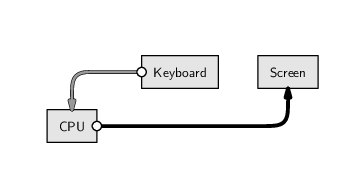
\includegraphics[width=0.5\linewidth]{img/script-commandline} \end{center}

\begin{center}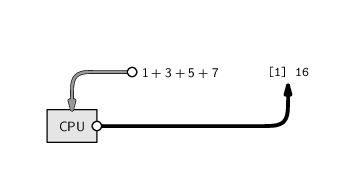
\includegraphics[width=0.5\linewidth]{img/script-commandlinedata} \end{center}

\begin{itemize}
\tightlist
\item
  Note que o resultado é apenas mostrado na tela, nada é salvo na
  memória (por enquanto)
\end{itemize}

\subsection{O editor de scripts}\label{o-editor-de-scripts}

\begin{itemize}
\tightlist
\item
  Para criar rotinas computacionais é necessário utilizar um editor de
  scripts.
\item
  Clique em
  \texttt{File\ \textgreater{}\ New\ file\ \textgreater{}\ R\ script}.
  Salve com a extensão \texttt{.R}.
\item
  Para enviar comandos diretamente para o console, selecione-os e aperte
  \texttt{Ctrl\ +\ \textless{}Enter\textgreater{}}.
\item
  Para adicionar comentários ao script, utiliza-se o símbolo \texttt{\#}
  antes do texto e/ou comandos. O que estiver depois do símbolo não será
  interpretado pelo R. Portanto:
\end{itemize}

\begin{Shaded}
\begin{Highlighting}[]
\DecValTok{2} \OperatorTok{+}\StringTok{ }\DecValTok{2}     \CommentTok{# esta linha será executada}
\CommentTok{# 2 + 2     esta linha não será executada}
\end{Highlighting}
\end{Shaded}

\subsection{Operadores aritméticos}\label{operadores-aritmeticos}

\begin{longtable}[]{@{}ll@{}}
\toprule
Operador & Significado\tabularnewline
\midrule
\endhead
\texttt{+} & adição\tabularnewline
\texttt{-} & subtração\tabularnewline
\texttt{*} & multiplicação\tabularnewline
\texttt{/} & divisão\tabularnewline
\texttt{\^{}} & potência\tabularnewline
\texttt{exp()} & exponencial\tabularnewline
\texttt{sqrt()} & raíz quadrada\tabularnewline
\texttt{factorial()} & fatorial\tabularnewline
\texttt{log()}; \texttt{log2()}; \texttt{log10()} &
logaritmos\tabularnewline
\bottomrule
\end{longtable}

\subsection{Ordens de execução}\label{ordens-de-execucao}

As operações são realizadas sempre seguindo as prioridades:

\begin{enumerate}
\def\labelenumi{\arabic{enumi}.}
\tightlist
\item
  De dentro para fora de parênteses \texttt{()}
\item
  Multiplicação e divisão
\item
  Adição e subtração
\end{enumerate}

\begin{Shaded}
\begin{Highlighting}[]
\OperatorTok{>}\StringTok{ }\DecValTok{5} \OperatorTok{*}\StringTok{ }\DecValTok{2} \OperatorTok{-}\StringTok{ }\DecValTok{10} \OperatorTok{+}\StringTok{ }\DecValTok{7}
\NormalTok{[}\DecValTok{1}\NormalTok{] }\DecValTok{7}
\OperatorTok{>}\StringTok{ }\DecValTok{5} \OperatorTok{*}\StringTok{ }\DecValTok{2} \OperatorTok{-}\StringTok{ }\NormalTok{(}\DecValTok{10} \OperatorTok{+}\StringTok{ }\DecValTok{7}\NormalTok{)}
\NormalTok{[}\DecValTok{1}\NormalTok{] }\OperatorTok{-}\DecValTok{7}
\OperatorTok{>}\StringTok{ }\DecValTok{5} \OperatorTok{*}\StringTok{ }\NormalTok{(}\DecValTok{2} \OperatorTok{-}\StringTok{ }\DecValTok{10} \OperatorTok{+}\StringTok{ }\DecValTok{7}\NormalTok{)}
\NormalTok{[}\DecValTok{1}\NormalTok{] }\OperatorTok{-}\DecValTok{5}
\OperatorTok{>}\StringTok{ }\DecValTok{5} \OperatorTok{*}\StringTok{ }\NormalTok{(}\DecValTok{2} \OperatorTok{-}\StringTok{ }\NormalTok{(}\DecValTok{10} \OperatorTok{+}\StringTok{ }\DecValTok{7}\NormalTok{))}
\NormalTok{[}\DecValTok{1}\NormalTok{] }\OperatorTok{-}\DecValTok{75}
\end{Highlighting}
\end{Shaded}

\subsection*{Exercícios}\label{exercicios}


\begin{enumerate}
\def\labelenumi{\arabic{enumi}.}
\tightlist
\item
  Calcule a seguinte equação: \(32 + 16^2 - 25^3\)
\item
  Divida o resultado por \(345\)
\item
  Qual o resultado da expressão \(\frac{e^{-2} 2^{4} - 1}{4!}\)?
\item
  E do logaritmo desta expressão?
\end{enumerate}

\subsection{\texorpdfstring{``Salvando''
resultados}{Salvando resultados}}\label{salvando-resultados}

Do exercício anterior

\begin{Shaded}
\begin{Highlighting}[]
\OperatorTok{>}\StringTok{ }\NormalTok{x <-}\StringTok{ }\DecValTok{32} \OperatorTok{+}\StringTok{ }\DecValTok{16}\OperatorTok{^}\DecValTok{2} \OperatorTok{-}\StringTok{ }\DecValTok{25}\OperatorTok{^}\DecValTok{3}
\OperatorTok{>}\StringTok{ }\NormalTok{x}
\NormalTok{[}\DecValTok{1}\NormalTok{] }\OperatorTok{-}\DecValTok{15337}
\OperatorTok{>}\StringTok{ }\NormalTok{x}\OperatorTok{/}\DecValTok{345}
\NormalTok{[}\DecValTok{1}\NormalTok{] }\OperatorTok{-}\FloatTok{44.45507}
\OperatorTok{>}\StringTok{ }\NormalTok{(y <-}\StringTok{ }\NormalTok{(}\KeywordTok{exp}\NormalTok{(}\OperatorTok{-}\DecValTok{2}\NormalTok{) }\OperatorTok{*}\StringTok{ }\DecValTok{2}\OperatorTok{^}\DecValTok{4} \OperatorTok{-}\StringTok{ }\DecValTok{1}\NormalTok{)}\OperatorTok{/}\KeywordTok{factorial}\NormalTok{(}\DecValTok{4}\NormalTok{))}
\NormalTok{[}\DecValTok{1}\NormalTok{] }\FloatTok{0.04855686}
\OperatorTok{>}\StringTok{ }\KeywordTok{log}\NormalTok{(y)}
\NormalTok{[}\DecValTok{1}\NormalTok{] }\OperatorTok{-}\FloatTok{3.02502}
\end{Highlighting}
\end{Shaded}

Quando criamos uma variável (\texttt{x}, \texttt{y}), ela fica
armazenada \textbf{temporariamente} na memória RAM.

\begin{center}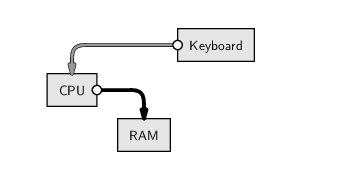
\includegraphics[width=0.5\linewidth]{img/script-assign} \end{center}

Para saber quais objetos estão criados, usamos a \textbf{função}
\texttt{ls()}

\begin{Shaded}
\begin{Highlighting}[]
\OperatorTok{>}\StringTok{ }\KeywordTok{ls}\NormalTok{()}
\NormalTok{[}\DecValTok{1}\NormalTok{] }\StringTok{"x"} \StringTok{"y"}
\end{Highlighting}
\end{Shaded}

Estas variáveis ficam armazenadas no chamado \emph{workspace} do R

\begin{itemize}
\tightlist
\item
  O \emph{workspace} consiste de tudo que or criado durante uma sessão
  do R, armazenado na memória RAM
\end{itemize}

Para efetivamente salvar esas variáveis, podemos armazenar esse
\emph{workspace} do R em disco, em um arquivo chamdo \texttt{.Rdata}

\begin{center}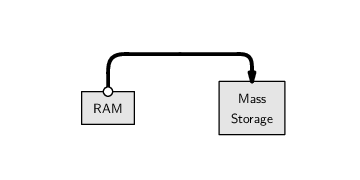
\includegraphics[width=0.5\linewidth]{img/script-workspace} \end{center}

\begin{center}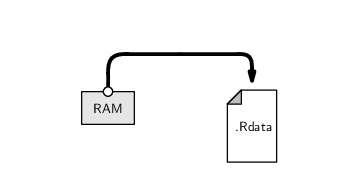
\includegraphics[width=0.5\linewidth]{img/script-workspacedata} \end{center}

\begin{itemize}
\tightlist
\item
  Quando o R é iniciado em um diretório com um arquivo \texttt{.Rdata},
  as variáveis salvas são automaticamente carregadas
\item
  No entanto, é sempre melhor salvar os dados e o \textbf{script}, assim
  é possível gerar os resultados novamente, sem salvar nada sem
  necessidade
\item
  Veremos mais pra frente como salvar variáveis específicas, por
  exemplo, resultados de uma análise que leva muito tempo para ser
  executada
\item
  O mais importante é salvar o \textbf{código}, assim sabemos
  \textbf{como} chegamos a determinado resultado, e podemos recriá-lo
  depois
\end{itemize}

\subsection{Finalizando o programa}\label{finalizando-o-programa}

A qualquer momento durante uma sessão você pode usar o comando

\begin{Shaded}
\begin{Highlighting}[]
\OperatorTok{>}\StringTok{ }\KeywordTok{save.image}\NormalTok{()}
\end{Highlighting}
\end{Shaded}

No RStudio:

\begin{itemize}
\tightlist
\item
  \texttt{File\ \textgreater{}\ Save\ As...}
\item
  Na janela que abrir, digite o nome do arquivo (por exemplo
  \texttt{script\_aula1}) e salve
\item
  Automaticamente o script será salvo com a extensão \texttt{.R} (nesse
  caso \texttt{script\_aula1.R}) no diretório de trabalho que você
  configurou no início
\end{itemize}

Alternativamente, você pode também salvar toda sua área de trabalho,
clicando em
\texttt{Workspace\ \textgreater{}\ Save\ As\ Default\ Workspace}. Este
processo irá gerar dois arquivos:

\begin{itemize}
\tightlist
\item
  \texttt{.Rdata}: contém todos os objetos criados durante uma sessão.
  Não é necessário (e nem recomendado) dar um nome antes do ponto. Dessa
  forma, a próxima vez que o programa for iniciado neste diretório, a
  área de trabalho será carregada automaticamente.
\item
  \texttt{.Rhistory}: um arquivo texto que contém todos os comandos que
  foram digitados no console.
\end{itemize}

\section*{Referências}\label{referencias}


\begin{itemize}
\tightlist
\item
  Leek, J. \href{https://leanpub.com/datastyle}{The Elements of Data
  Analytic Style}. Leanpub, 2015.
\item
  Murrell, P.
  \href{https://www.stat.auckland.ac.nz/~paul/ItDT/HTML}{Introduction to
  data technologies}. Boca Raton: Chapman \& Hall/CRC, 2009.
\item
  Peng, RD. \href{https://leanpub.com/rprogramming}{R programming for
  data science}. Leanpub, 2015.
\end{itemize}

\end{document}
